\input{../../latex/preamble.tex}

\usepackage{tikz}
\usetikzlibrary{positioning,shapes.geometric}

\tikzset{
  pregunta/.style={draw, rounded corners, fill=blue!10, align=center, font=\small},
  hoja/.style={draw, fill=green!15, align=center, font=\small},
  hojano/.style={draw, fill=red!15, align=center, font=\small},
  claseA/.style={circle, fill=blue!60, inner sep=2pt},
  claseB/.style={rectangle, fill=red!70, inner sep=2.5pt},
}

\title{Sesión 4: Árboles de Decisión, kNN y SVM}
\subtitle{Tres formas distintas de clasificar}
\date{}

\begin{document}

\frame{\titlepage}

\begin{frame}{Qué vimos hasta ahora?}
  \begin{itemize}
    \item Regresión lineal, una frontera de decisión \textbf{recta} (o un hiperplano)
    \item Hoy: tres modelos con nuevas visiones sobre el problema
  \end{itemize}
  \vspace{0.5em}
  \begin{center}
    \begin{tabular}{ll}
      \toprule
      Modelo & Idea \\
      \midrule
      Árbol de decisión & Hacer preguntas de sí o no muy seguidas\\
      kNN & Mirar a los vecinos más cercanos \\
      SVM & Separar las clases con el hiperplano más ancho posible \\
      \bottomrule
    \end{tabular}
  \end{center}
\end{frame}

\part{Árboles de decisión}
\frame{\partpage}

\section{¿Qué es un árbol de decisión?}

\begin{frame}{Ya lo hemos visto}
  \ejemplo{
    \textbf{¿Quién es quién?} o \textbf{Akinator}: para adivinar un
    personaje hacemos preguntas de sí o no. Las buenas preguntas descartan
    a mucha gente, las malas descartan a uno
    solo.
  }
  \pause
  \definicion{
    Un \textbf{árbol de decisión} es un modelo que clasifica haciendo una
    secuencia de preguntas sobre las features. Cada respuesta nos manda
    por una rama distinta, hasta llegar a una predicción.
  }
  Entrenar el árbol es descubrir \textbf{qué preguntas hacer y en qué
  orden}.
\end{frame}

\begin{frame}{¿Fulbo?}
  \begin{center}
    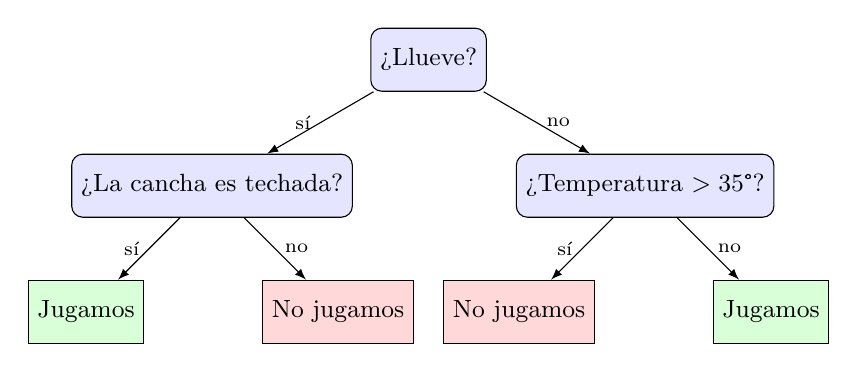
\begin{tikzpicture}[level distance=1.6cm,
        level 1/.style={sibling distance=5.5cm},
        level 2/.style={sibling distance=3.2cm},
        edge from parent/.style={draw, -latex},
        every node/.style={minimum height=0.8cm}]
      \node[pregunta] {¿Llueve?}
        child {node[pregunta] {¿La cancha es techada?}
          child {node[hoja] {Jugamos} edge from parent node[left, font=\scriptsize] {sí}}
          child {node[hojano] {No jugamos} edge from parent node[right, font=\scriptsize] {no}}
          edge from parent node[left, font=\scriptsize] {sí}}
        child {node[pregunta] {¿Temperatura $> 35$°?}
          child {node[hojano] {No jugamos} edge from parent node[left, font=\scriptsize] {sí}}
          child {node[hoja] {Jugamos} edge from parent node[right, font=\scriptsize] {no}}
          edge from parent node[right, font=\scriptsize] {no}};
    \end{tikzpicture}
  \end{center}
  \begin{itemize}
    \item \textbf{Nodo raíz}: la primera pregunta. \textbf{Nodos internos}:
      preguntas intermedias. \textbf{Hojas}: la predicción final.
    \item \textbf{Profundidad}: cuántas preguntas hay, como máximo, desde la
      raíz hasta una hoja (acá, 2).
  \end{itemize}
\end{frame}

\begin{frame}{Preguntas sobre features numéricas}
  \begin{itemize}
    \item Con una feature categórica la pregunta es evidente: ``¿llueve?''
    \item Con una numérica el árbol elige un \textbf{umbral}: ``¿temperatura
      $\leq 35$?'', ``¿edad $\leq 17.5$?''
    \item Cada pregunta corta el espacio con una línea \textbf{paralela a un
      eje}
  \end{itemize}
\end{frame}

\section{¿Cómo elige las preguntas?}

\begin{frame}{Que cada grupo quede lo más limpio posible}
  \begin{itemize}
    \item Arrancamos con todos los datos en la raíz
    \item Probamos \textbf{todas} las preguntas posibles (cada feature, cada
      umbral)
    \item Nos quedamos con la que deja los dos grupos más limpios, cada uno
      con casi todos los ejemplos de una misma clase
    \item Repetimos lo mismo dentro de cada grupo, y así hasta terminar
  \end{itemize}
  \pause
  \definicion{
    Un nodo es \textbf{puro} si todos sus ejemplos son de la misma clase.
    Para elegir preguntas necesitamos un número que mida qué tan
    \textbf{impuro} es un nodo.
  }
\end{frame}

\begin{frame}{Impureza de Gini}
  \definicion{
    Si $p_k$ es la proporción de ejemplos de la clase $k$ en un nodo:
    $$\text{Gini} = 1 - \sum_k p_k^2$$
  }
  Es decir: la probabilidad de equivocarse si etiquetamos un ejemplo
  al azar siguiendo las proporciones del nodo.
  \begin{itemize}
    \item 10 ``sí'', 0 ``no'': $\text{Gini} = 1 - (1^2 + 0^2) = 0$
      \quad (puro)
    \item 5 ``sí'', 5 ``no'': $\text{Gini} = 1 - (0.5^2 + 0.5^2) = 0.5$
      \quad (lo más mezclado posible)
    \item 8 ``sí'', 2 ``no'': $\text{Gini} = 1 - (0.8^2 + 0.2^2) = 0.32$
  \end{itemize}
\end{frame}

\begin{frame}{Entropía}
  \definicion{
    Otra forma de medir el desorden (cortesía de la teoría de la información):
    $$H = -\sum_k p_k \log_2 p_k$$
  }
  \begin{itemize}
    \item Nodo puro: $H = 0$
    \item 50/50 entre dos clases: $H = 1$ (``un bit'' de incertidumbre)
  \end{itemize}
  \pause
  \importante{
    En la práctica Gini y entropía casi siempre eligen las mismas
    preguntas. scikit-learn usa Gini por defecto
    (\texttt{criterion=\textquotedbl{}gini\textquotedbl{}}); se puede cambiar con
    \texttt{criterion=\textquotedbl{}entropy\textquotedbl{}}.
  }
\end{frame}

\begin{frame}{Eligiendo la mejor pregunta: un ejemplo}
  10 días: 6 jugamos, 4 no. \quad Gini de la raíz $= 1 - (0.6^2 + 0.4^2) = 0.48$
  \vspace{0.5em}
  \begin{columns}[T]
    \begin{column}{0.48\textwidth}
      \textbf{Pregunta A: ¿Llueve?}
      \begin{itemize}
        \item Sí (4 días): 1 jugamos, 3 no \\ Gini $= 0.375$
        \item No (6 días): 5 jugamos, 1 no \\ Gini $\approx 0.278$
      \end{itemize}
    \end{column}
    \begin{column}{0.48\textwidth}
      \textbf{Pregunta B: ¿Hace frío?}
      \begin{itemize}
        \item Sí (5 días): 3 jugamos, 2 no \\ Gini $= 0.48$
        \item No (5 días): 3 jugamos, 2 no \\ Gini $= 0.48$
      \end{itemize}
    \end{column}
  \end{columns}
  \vspace{0.5em}
  \pause
  Promedio ponderado por cantidad de ejemplos:
  \begin{itemize}
    \item A: $0.4 \cdot 0.375 + 0.6 \cdot 0.278 \approx 0.317$
    \item B: $0.5 \cdot 0.48 + 0.5 \cdot 0.48 = 0.48$ \quad (¡no mejoró
      nada!)
  \end{itemize}
  Gana ``¿Llueve?'': es la pregunta que más reduce la impureza.
\end{frame}

\section{Overfitting en árboles}

\begin{frame}{¿Cuándo dejamos de preguntar?}
  Si no lo frenamos, el árbol sigue preguntando hasta que \textbf{todas}
  las hojas son puras.
  \pause
  \importante{
    Un árbol sin límites \textbf{memoriza} el set de entrenamiento: llega a
    100\% de accuracy en train y le va bastante peor en test. Eso es
    \textbf{overfitting}.
  }
  Hiperparámetros para frenarlo:
  \begin{itemize}
    \item \texttt{max\_depth}: profundidad máxima
    \item \texttt{min\_samples\_leaf}: mínima cantidad de ejemplos por hoja
    \item \texttt{min\_samples\_split}: mínima cantidad de ejemplos para partir un nodo
  \end{itemize}
\end{frame}

\begin{frame}{Hiperparámetros vs. parámetros}
  \definicion{
    Los \textbf{parámetros} los aprende el modelo al entrenar (las preguntas
    y umbrales del árbol, los $w$ de la regresión). Los
    \textbf{hiperparámetros} los elegimos nosotros \textbf{antes} de
    entrenar (\texttt{max\_depth}, el learning rate).
  }
  \ejemplo{
    \texttt{max\_depth=1}: una sola pregunta, el modelo es demasiado simple
    (\textbf{underfitting}). \texttt{max\_depth=None}: memoriza todo
    (\textbf{overfitting}). El punto justo está en el medio, y lo
    encontramos probando y mirando el resultado en datos que el modelo no
    vio.
  }
\end{frame}

\section{Ventajas y desventajas}

\begin{frame}{Lo bueno y lo malo de los árboles}
  \begin{columns}[T]
    \begin{column}{0.48\textwidth}
      \textbf{Lo bueno}
      \begin{itemize}
        \item Se pueden \textbf{leer} y explicar: son reglas de sí o no
        \item No necesitan escalar los datos
        \item Capturan relaciones no lineales
        \item Dicen qué features usaron más (\emph{feature importance})
      \end{itemize}
    \end{column}
    \begin{column}{0.48\textwidth}
      \textbf{Lo malo}
      \begin{itemize}
        \item Tienden muchísimo al overfitting
        \item Son \textbf{inestables}: cambiar unos pocos datos puede cambiar
          todo el árbol
        \item Fronteras en escalones, torpes para cortes diagonales
      \end{itemize}
    \end{column}
  \end{columns}
  \pause
  \vspace{0.5em}
  \ejemplo{
    \textbf{Random Forest}: entrenar cientos de árboles distintos y que
    voten. Corrige gran parte de lo malo, y es de los modelos más usados en
    la industria para datos en tablas.
  }
\end{frame}

\section{Árboles en código}

\begin{frame}[fragile]{Árboles de decisión con scikit-learn}
  \begin{lstlisting}[language=Python]
from sklearn.tree import DecisionTreeClassifier, plot_tree

modelo = DecisionTreeClassifier(max_depth=3, random_state=0)
modelo.fit(X_train, y_train)

modelo.score(X_test, y_test)    # accuracy
modelo.feature_importances_     # cuanto aporto cada feature

plot_tree(modelo, feature_names=X.columns, filled=True)
  \end{lstlisting}
  La interfaz es la misma de siempre: \texttt{fit}, \texttt{predict},
  \texttt{score}. Cambia lo que pasa adentro.
\end{frame}

\part{kNN y SVM}
\frame{\partpage}

\section{k vecinos más cercanos (kNN)}

\begin{frame}{Aprendiendo de los vecinos}
  \definicion{
    \textbf{kNN} (\emph{k-Nearest Neighbors}) clasifica un punto nuevo
    mirando los $k$ ejemplos de entrenamiento más cercanos y eligiendo la
    clase que más se repite entre ellos (votación).
  }
  \begin{columns}[c]
    \begin{column}{0.5\textwidth}
      \begin{enumerate}
        \item Llega un punto nuevo
        \item Calcular la distancia a \textbf{todos} los puntos de train
        \item Quedarse con los $k$ más cercanos
        \item Votar
      \end{enumerate}
    \end{column}
    \begin{column}{0.45\textwidth}
      \begin{center}
        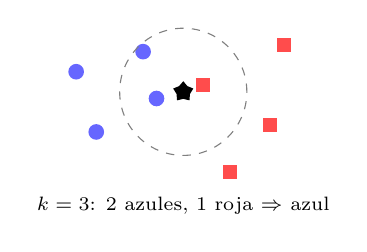
\begin{tikzpicture}[scale=0.85]
          \node[claseA] at (0.3,1.8) {};
          \node[claseA] at (1.3,2.1) {};
          \node[claseA] at (0.6,0.9) {};
          \node[claseA] at (1.5,1.4) {};
          \node[claseB] at (3.2,1.0) {};
          \node[claseB] at (2.6,0.3) {};
          \node[claseB] at (3.4,2.2) {};
          \node[claseB] at (2.2,1.6) {};
          \draw[dashed, gray] (1.9,1.5) circle (0.95);
          \node[star, star points=5, fill=black, inner sep=1.8pt] at (1.9,1.5) {};
          \node[font=\scriptsize] at (1.9,-0.2) {$k=3$: 2 azules, 1 roja $\Rightarrow$ azul};
        \end{tikzpicture}
      \end{center}
    \end{column}
  \end{columns}
\end{frame}

\begin{frame}{Distancia}
  La distancia más usada es la \textbf{euclídea}:
  $$d(\mathbf{a}, \mathbf{b}) = \sqrt{(a_1 - b_1)^2 + (a_2 - b_2)^2 + \dots + (a_n - b_n)^2}$$
  \pause
  \importante{
    Si una feature es ``edad'' (0 a 100) y otra es ``sueldo'' (0 a
    3.000.000), el sueldo domina por completo la distancia y la edad no
    cuenta para nada. Con kNN \textbf{siempre hay que escalar} los datos
    antes de entrenar.
  }
\end{frame}

\begin{frame}{¿Qué $k$ elegimos?}
  \begin{itemize}
    \item \textbf{$k = 1$}: copia la clase del vecino más cercano. Frontera
      muy irregular, sensible al ruido $\Rightarrow$ overfitting
    \item \textbf{$k$ muy grande}: siempre
      predice la clase mayoritaria $\Rightarrow$ underfitting
    \item En el medio está el punto justo
  \end{itemize}
  \pause
  \ejemplo{
    $k$ es un hiperparámetro, igual que \texttt{max\_depth}. Se suele usar
    un $k$ impar para evitar empates cuando hay dos clases.
  }
\end{frame}

\begin{frame}{Lo bueno y lo malo}
  \begin{columns}[T]
    \begin{column}{0.48\textwidth}
      \textbf{Lo bueno}
      \begin{itemize}
        \item Idea simple y fácil de explicar
        \item ``Entrenar'' es rápido: solo guarda los datos
        \item Fronteras tan complicadas como haga falta
      \end{itemize}
    \end{column}
    \begin{column}{0.48\textwidth}
      \textbf{Lo malo}
      \begin{itemize}
        \item Predecir es \textbf{lento}: compara contra todo el train
        \item Obligatorio escalar
        \item Funciona mal con muchísimas features (en dimensiones altas
          ``todos están lejos de todos'')
      \end{itemize}
    \end{column}
  \end{columns}
  \vspace{0.5em}
  \definicion{
    A kNN se le llama \textbf{lazy learner} porque no aprende nada al
    entrenar, deja todo el trabajo para el momento de predecir.
  }
\end{frame}

\begin{frame}[fragile]{kNN con scikit-learn}
  \begin{lstlisting}[language=Python]
from sklearn.neighbors import KNeighborsClassifier
from sklearn.preprocessing import StandardScaler

scaler = StandardScaler()
X_train_esc = scaler.fit_transform(X_train)
X_test_esc = scaler.transform(X_test)

modelo = KNeighborsClassifier(n_neighbors=5)
modelo.fit(X_train_esc, y_train)
modelo.score(X_test_esc, y_test)
  \end{lstlisting}
\end{frame}

\section{Máquinas de vectores de soporte (SVM)}

\begin{frame}{Volvemos a la idea de los hiperplanos}
  \begin{columns}[c]
    \begin{column}{0.5\textwidth}
      \begin{itemize}
        \item Si las clases se pueden separar con una recta, en general
          hay \textbf{infinitas} rectas que lo hacen
        \item La regresión logística elige una cualquiera de ellas
        \item SVM elige la que deja más espacio entre las
          dos clases
      \end{itemize}
    \end{column}
    \begin{column}{0.45\textwidth}
      \begin{center}
        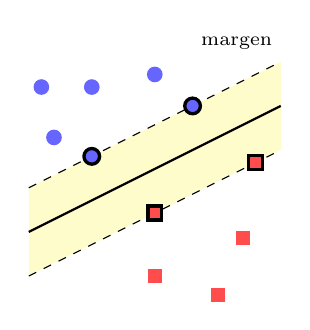
\begin{tikzpicture}[scale=0.8]
          \fill[yellow!20] (0,0.6) -- (0,2.0) -- (4,4.0) -- (4,2.6) -- cycle;
          \draw[thick] (0,1.3) -- (4,3.3);
          \draw[dashed] (0,0.6) -- (4,2.6);
          \draw[dashed] (0,2.0) -- (4,4.0);
          \node[claseA] at (0.4,2.8) {};
          \node[claseA] at (1.0,3.6) {};
          \node[claseA] at (2.0,3.8) {};
          \node[claseA] at (0.2,3.6) {};
          \node[claseA, draw=black, very thick] at (1.0,2.5) {};
          \node[claseA, draw=black, very thick] at (2.6,3.3) {};
          \node[claseB] at (2.0,0.6) {};
          \node[claseB] at (3.4,1.2) {};
          \node[claseB] at (3.0,0.3) {};
          \node[claseB, draw=black, very thick] at (2.0,1.6) {};
          \node[claseB, draw=black, very thick] at (3.6,2.4) {};
          \node[font=\scriptsize] at (3.3,4.3) {margen};
        \end{tikzpicture}
      \end{center}
    \end{column}
  \end{columns}
\end{frame}

\begin{frame}{Margen y vectores de soporte}
  \definicion{
    El \textbf{margen} es el ancho de la separación entre las dos clases. SVM
    busca el hiperplano que \textbf{maximiza el margen}.
  }
  \definicion{
    Los \textbf{vectores de soporte} son los puntos que quedan justo en el
    borde de la separación (los remarcados en el dibujo). Son los únicos que
    determinan la frontera: si movemos cualquier otro punto, la frontera
    no cambia.
  }
  Intuición: una separación más ancha deja más espacio de seguridad para datos
  nuevos que caigan cerca de la frontera.
\end{frame}

\begin{frame}{Margen blando: el hiperparámetro $C$}
  En datos reales casi nunca hay una calle perfectamente vacía. Siempre
  hay algún punto ruidoso del lado equivocado.
  \begin{itemize}
    \item SVM permite que algunos puntos invadan la separación, con una
      penalización
    \item \textbf{$C$ grande}: casi no tolera errores, separación angosta, riesgo
      de overfitting
    \item \textbf{$C$ chico}: tolera más errores, separación ancha, modelo más
      simple
  \end{itemize}
  \pause
  \importante{
    Otra vez lo mismo: un hiperparámetro que maneja cuánto se
    acomoda el modelo a los datos de entrenamiento.
  }
\end{frame}

\begin{frame}{¿Y si no se pueden separar con una recta?}
  \begin{columns}[c]
    \begin{column}{0.48\textwidth}
      \begin{center}
        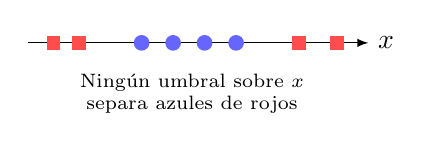
\begin{tikzpicture}[scale=0.8]
          \draw[-latex] (-2.6,0) -- (2.8,0) node[right] {$x$};
          \foreach \x in {-2.2,-1.8,1.7,2.3} \node[claseB] at (\x,0) {};
          \foreach \x in {-0.8,-0.3,0.2,0.7} \node[claseA] at (\x,0) {};
          \node[font=\scriptsize, align=center] at (0,-0.8) {Ningún umbral sobre $x$\\separa azules de rojos};
        \end{tikzpicture}
      \end{center}
    \end{column}
    \pause
    \begin{column}{0.48\textwidth}
      \begin{center}
        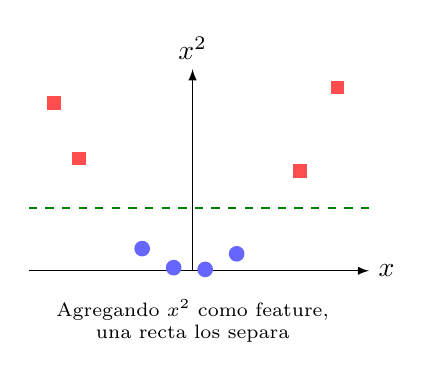
\begin{tikzpicture}[scale=0.8]
          \draw[-latex] (-2.6,0) -- (2.8,0) node[right] {$x$};
          \draw[-latex] (0,0) -- (0,3.2) node[above] {$x^2$};
          \foreach \x in {-2.2,-1.8,1.7,2.3} \node[claseB] at (\x,{0.55*\x*\x}) {};
          \foreach \x in {-0.8,-0.3,0.2,0.7} \node[claseA] at (\x,{0.55*\x*\x}) {};
          \draw[thick, dashed, green!50!black] (-2.6,1.0) -- (2.8,1.0);
          \node[font=\scriptsize, align=center] at (0,-0.8) {Agregando $x^2$ como feature,\\una recta los separa};
        \end{tikzpicture}
      \end{center}
    \end{column}
  \end{columns}
  \vspace{0.5em}
  Idea: llevar los datos a un espacio con más dimensiones, donde sí se
  puedan separar con una recta (o un plano).
\end{frame}

\begin{frame}{El trucazo del kernel}
  \definicion{
    Un \textbf{kernel} le permite a SVM trabajar \emph{como si} los datos
    estuvieran en un espacio de más dimensiones, sin tener que calcular
    esas nuevas features de verdad.
  }
  \begin{itemize}
    \item \texttt{kernel=\textquotedbl{}linear\textquotedbl{}}: frontera recta, como la logística
    \item \texttt{kernel=\textquotedbl{}poly\textquotedbl{}}: fronteras polinómicas (curvas)
    \item \texttt{kernel=\textquotedbl{}rbf\textquotedbl{}}: el más usado. Fronteras muy flexibles, que
      pueden encerrar regiones (círculos, islas)
  \end{itemize}
  \pause
  \importante{
    SVM también usa distancias, así que también hay que escalar
    los datos!!!
  }
\end{frame}

\begin{frame}[fragile]{SVM con scikit-learn}
  \begin{lstlisting}[language=Python]
from sklearn.svm import SVC

modelo = SVC(kernel="rbf", C=1.0)
modelo.fit(X_train_esc, y_train)

modelo.score(X_test_esc, y_test)
modelo.support_vectors_      # los vectores de soporte
  \end{lstlisting}
  SVM fue \emph{el} modelo estrella antes de que llegaran las redes
  neuronales profundas, y sigue funcionando muy bien con datasets
  medianos.
\end{frame}

\section{Comparando los modelos}

\begin{frame}{¿Cuál uso?}
  \begin{center}
    \small
    \begin{tabular}{lcccc}
      \toprule
      & Logística & Árbol & kNN & SVM \\
      \midrule
      Frontera & recta & escalones & libre & recta o curva \\
      ¿Hay que escalar? & conviene & no & sí & sí \\
      ¿Se puede interpretar? & bastante & mucho & poco & poco \\
      Velocidad al predecir & rápida & rápida & lenta & media \\
      Hiperparámetro clave & $C$ & \texttt{max\_depth} & $k$ & $C$, kernel \\
      \bottomrule
    \end{tabular}
  \end{center}
  \pause
  \importante{
    No hay un modelo que gane siempre. La única forma
    de saber cuál anda mejor en un problema es probar varios y
    compararlos en datos que no vieron.
  }
\end{frame}

\begin{frame}{Resumen}
  \begin{itemize}
    \item Árbol de decisión: preguntas de sí o no elegidas para que cada
      grupo quede lo más puro posible (Gini o entropía)
    \item kNN: clasificar por votación de los $k$ vecinos más cercanos
    \item SVM: la frontera con el margen más ancho; con kernels, también
      fronteras curvas
    \item Los tres tienen hiperparámetros que regulan el equilibrio entre
      underfitting y overfitting
  \end{itemize}
  \vspace{1em}
  \centering
  \Large ¿Preguntas?
\end{frame}

\end{document}
